\documentclass[a4paper,12pt,leqno]{article}
\usepackage[utf8]{inputenc}
\usepackage[T1]{fontenc}
\usepackage[polish]{babel}
\usepackage{amsmath}
\usepackage{a4wide}
\usepackage{graphicx}
\usepackage{subfig}
\usepackage{wrapfig}
\usepackage{program}

\title{\textbf{Algorytmy ewolucyjne}\\
       {\Large Raport z zadania pierwszego}\\[-1ex]}
\author{Karol Konaszyński i Wiktor Janas}
\date{Wrocław, dnia \today\ r.}

\begin{document}
\maketitle

\newcommand{\avg}{\mathrm{avg}}
\newcommand{\dist}{\mathrm{dist}}
\newcommand{\median}{\mathrm{median}}
\newcommand{\target}{\mathrm{target}}
\newcommand{\RETURN}{|return|\ }

Tematem tego projektu jest zastosowanie algorytmów ewolucyjnych do rozpoznawania obrazów. 
Problem rozpoznawania obrazów ma liczne zastosowania: od analizy zdjęć satelitarnych poprzez monitorowanie ruchu drogowego, po przemysł filmowy.
Z drugiej rozwiązanie go okazuje się być trudne, a pojęcie ,,podobieństwa obrazów'', oczywiste dla człowieka, nie jest precyzyjnie zdefiniowane.
Podejście zaproponowane w tej pracy polega na analizie samego kształtu obrazu, który uzyskujemy poprzez analizę jasności poszczególnych
pikseli (z pominięciem informacji o kolorze).

Przyjęliśmy następujące założenia: dana jest baza obrazów o zadanych nazwach (to znaczy, że wiemy, co one przedstawiają).
Każdy obraz, który chcemy rozpoznać (zapytanie) jest przyrównywane dp wszystkich obrazów z bazy.
Spośród obrazów bazowych wybieramy te, których odległość do zapytania jest najmniejsza.

\section{Znajdowanie punktów charakterystycznych}
Pierwszym etapem przetwarzania obrazu (pochodzącego z bazy danych lub będącego zapytaniem) jest znalezienie na nim punktów charakterystycznych.
Niech $\avg(x,y,d)$ oznacza średnią jasność obrazu w kwadracie o środku w $(x,y)$ i boku długości $d$. Dla piksela o współrzędnych $(x_0,y_0)$ oraz danej
wartości $d$ można zdefiniować funkcję
\[ F_d(\alpha) = \avg(x_0,y_0,d) - \avg( x_0+d\sin\alpha, y_0+d\cos\alpha, d) \]
Intuicyjnie jest to gradient piksela $(x_0,y_0)$ w kierunku $\alpha$ na obrazie zmniejszonym $d$-krotnie. Przyjmując kilka ustalonych wartości $d$
(w naszej implementacji były to $1,3,8$), można zdefiniować funkcję
\[ G(\alpha) = \sqrt[3]{F_1(\alpha) \cdot F_3(\alpha) \cdot F_8(\alpha)} \]
Następnie można obliczyć amplitudę tej funkcji:
\[ A = \max_\alpha G(\alpha) - \min_\alpha G(\alpha) \]
Wartość tą przyjmujemy za ,,miarę ciekawości'' piksela. 

Intuicja stojąca za tym algorytmem jest prosta -- szukamy punktów, w otoczeniu których następuje zmiana jasności obrazu. Miarą zmiany jasności w danym
kierunku jest gradient, zatem funkcja $F$ opisuje zmianę jasności obrazu we wszystkich kierunkach. Musimy jednak wziąć pod uwagę, że niektóre zmiany są
jedynie lokalne. Aby wyeleminować szum, obliczamy średnią geometryczbą funkcję $F$ dla kilku skal (jest to funkcja $G$) -- jeżeli istotnie zachodzi
rozpatrywany piksel leży w obszarze silnych zmian, nastąpi rezonans, gdy natomiast zmiana jest lokalna, funkcja większej skali ją ,,wyciszy''.
Według naszej całkowicie subiektywnej oceny skale 1,3,8 spradzają się najlepiej.

Mając określoną miarę ciekawości każdego piksela, chcemy wybrać określoną liczbę punktów charakterystycznych, które będą opisywały kształt obiektu
(liczba ta jest parametrem alogorytmu, najczęściej przyjmowaliśmy 50). Do tego celu zastosowaliśmy następujący algorytm: w każdym kolejnym kroku wybieramy
najciekawszy piksel na obrazku i dodajemy go do zbioru punktów interesujących. Nastepnie pewne jego otoczenie oznaczamy jako tabu i powtarzamy procedurę tak
długo, aż wszystkie punkty zostaną tabu. Aby określić wielkość tabu, zastosowaliśmy heurystykę ,,im ciekawiej tym gęściej''. Mianowicie, wielkość tabu jest
odwrotnie proporcjonalna do miary ciekawości punktu z pewnym współczynnikiem, który jest dobierany (za pomocą wyszukiwania binarnego) tak, aby ostateczny
zbiór punktów żądaną określoną wielkość. Proces wyszukiwania ciekawych punktów ilustruje rysunek \ref{poisrch}.

\begin{figure}\centering
\subfloat[gradient, $d = 1$]{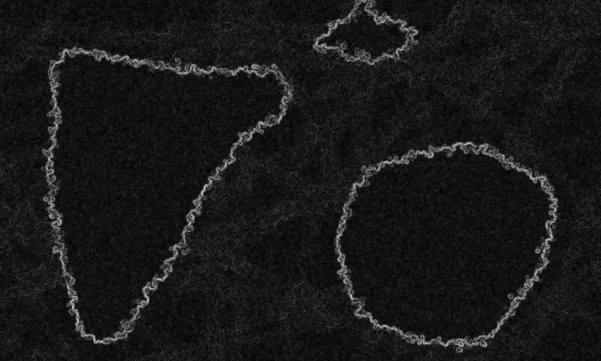
\includegraphics[width=6cm,keepaspectratio=true]{./noisy-grad-1.png}}\hspace{5mm}
\subfloat[gradient, $d = 3$]{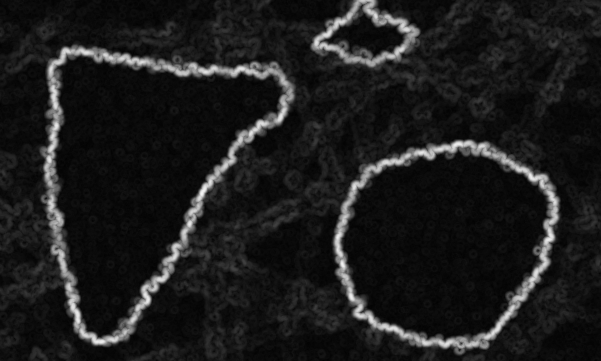
\includegraphics[width=6cm,keepaspectratio=true]{./noisy-grad-3.png}}\\
\subfloat[gradient, $d = 8$]{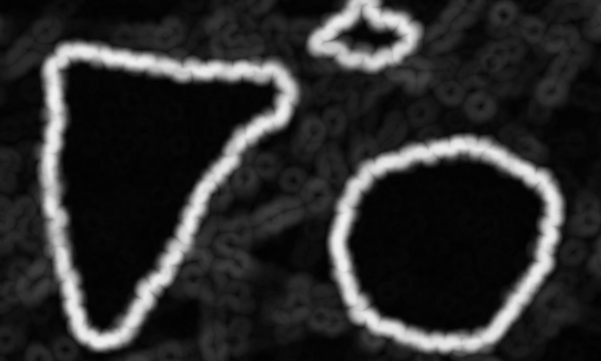
\includegraphics[width=6cm,keepaspectratio=true]{./noisy-grad-8.png}}\hspace{5mm}
\subfloat[gradient, łącznie]{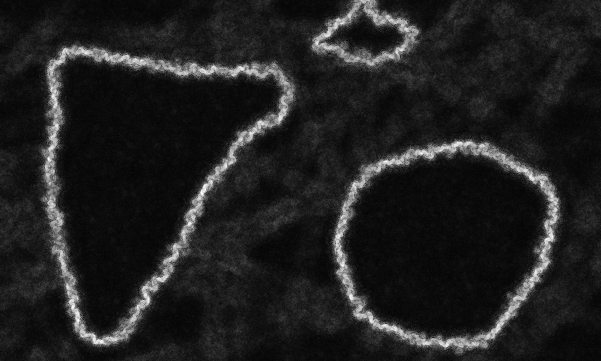
\includegraphics[width=6cm,keepaspectratio=true]{./noisy-grad.png}}\\
\subfloat[znalezione punkty]{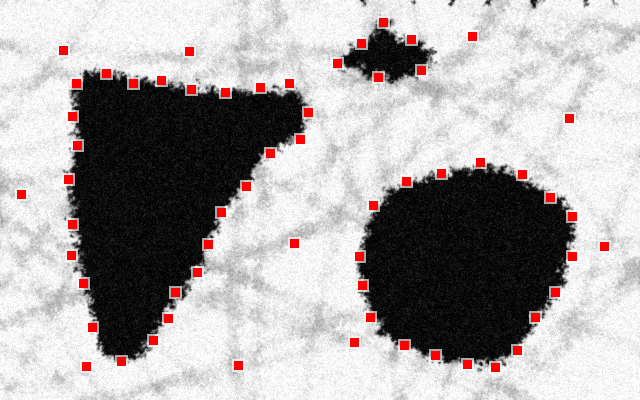
\includegraphics[width=6cm,keepaspectratio=true]{./noisy-pois.png}}
\caption{Proces wyszukiwania punktów charakterystycznych}\label{poisrch}
\end{figure}

\subsection{Zastosowanie ewolucji i kodowanie osobników}
Mając już punkty charakterystyczne, możemy zająć się badaniem podobienstwa obrazków. Mówimy, że obrazki są równoważne, jeżeli istnieje przekształcenie afiniczne 
przenoszące jeden na drugi. Miarą podobieństwa dwóch zbiorów punktów infimum, po wszystkich przekształceniach,
sumy ,,odległości,, jednego z nich od przekształconego drugiego oraz w drugą stronę. 
Odległość natomiast dwóch zbiorów definiujemy jako średnią odległość pomiędzy punktem z pierwszego zbioru a najbliższym mu punktem z drugiego, Formalniej,
\[
\mathrm{similar}(\bar{A}, \bar{B}) = \inf\{\textrm{dist}(\bar{A} - M\bar{B}) \;\arrowvert\; M\text{: afiniczne}\}
\]gdzie:
\[
\dist(\{a_1, \dots, a_m\}, \{b_1, \dots, b_n\}) = \frac{\sum_{i=1}^m \min_{j=1..n}(\|a_i - b_j\|)}{m} + \frac{\sum_{i=1}^n \min_{j=1 \dots m}(\|b_i - a_j\|)}{n}
\]
Jednak aby znaleźć wielkość $\mathrm{similar}$ musimy znaleźć przekształcenie minimalizujące odległość. I tutaj zastosujemy ewolucję. 
Naszymi osobnikami będą macierze afiniczne, czyli macierze postaci:
$\begin{pmatrix}
\star & \star & \star \\
\star & \star & \star \\
0 & 0 & 1
\end{pmatrix}$, gdzie drugi minor główny jest złożeniem obrotu i skalowania, natomiast ostatnia kolumna odpowiada za translację.
Funkcją celu jest zatem 
\[
\target = -\dist(\bar{q}, M\bar{b})
\]
gdzie $\bar{q}$ jest wektorem punktów charakterystycznych obrazka z zapytania, zaś $\bar{b}$ - wektorem tychże dla obrazka z bazy.
Celem ewolucji jest zmaksymalizowanie funkcji celu, czyli znalezienie przekształcenia minimalizującego odległość.

\subsection{Ewolucja}
Do niniejszego problemu wykorzystaliśmy ideę Differential Evolution. Pseudokod funkcji wykonującej ewolucję wygląda następująco:
\begin{figure}
\begin{program}
\FUNCT |evolve| \BODY
    P := \{\}
    \FOR i := 1 \TO N \DO
        P := P + |random_translation|() * |random_rotation|() * |random_scaling|()
    \END
    \WHILE \NOT |termination_condition|() \DO
        \FOR i := 1 \TO N \DO
            |evaluate|(P_i)
        \END
        |sort|(P) 
        ~
        P := \set{P_i | i \leq N*|replace\_rate| }
        \FOR i := 1 \TO N*|replace_rate| \DO
            \IF |random|(|de_prop|)
                \THEN P := P + |de_crossover|(P);
                \ELSE P := P + |roulette_selection|(P); \FI
        \END
        ~
        \FOR i := 1 \TO N \DO 
            \IF |random|(|t_prop|)
	        \THEN P_i := |random_translation| * P_i; \FI
            \IF |random|(|s_prop|)
                \THEN P_i := |random_scaling| * P_i; \FI
            \IF |random|(|r_prop|)
                \THEN P_i := |random_rotation| * P_i; \FI
        \END
    \END
\END

\FUNCT |de_crossover| \BODY
    x1 := |roulette_selection|(P)
    x2 := |roulette_selection|(P),\; x1 \neq x2
    x3 := |roulette_selection|(P),\; x3 \neq x1,\; x3 \geq x2
    \RETURN x1 + (x3-x2) * f_\text{de}
\END

\FUNCT |termination_condition| \BODY
    \RETURN |generation_index| > G \vee
            |max_target|(|generation_index|, |generation_index|-K) \geq
            |max_target|(|generation_index|-K, |generation_index|-2*K)
\END
\end{program}
\end{figure}

Skomentuję krótko działanie powyższych funkcji. Najpierw odbywa się losowa inicjacja populacji z parametrem N. Następnie wchodzimy w pętlę ewolucji,
która wykonuje się aż nie zostanie spełniony warunek zakończenia.
W pętli, pierwszą rzeczą jest ewaluacja każdego osobnika, czyli znalezienie dla niego wartości $\target$. 
Potem następuje zastąpienie części populacji przez osobniki bądź otrzymane w wyniku krzyżowania DE (z określonym jako parametr prawdopodobieństwem),
bądź wybrane na zasadzie ruletki z całości populacji (zjawisko generational gap).
Na końcu działania ciała pętli następuje mutacja każdego osobnika, czyli przemnożenie go (z lewej strony) przez macierz losowego przesunięcia, 
skalowania bądź obrotu, z prawdopodobieństwami określonymi jako globalne parametry algorytmu.
Warunkiem zakończenia jest natomiast przekroczenie pewnej ilości pokoleń (parametr algorytmu, zwykle rzędu 200) bądź stwierdzeniem, 
że w czasie ostatnich K pokoleń nie nastąpiła poprawa w stosunku do poprzednich K pokoleń (K jest również parametrem). Precyzyjniej, najlepszy osobnik z ostatnich 
K pokoleń okazał się nielepszy niż najlepszy z poprzednich K pokoleń.

Skomentuję jeszcze dwa miejsca w tym algorytmie.
Krzyżowanie DE polega na wybraniu, na zasadzie ruletki, trzech różnych osobników $x_1, x_2, x_3$ a następnie utworzeniu z nich osobnika postaci
$x1 + f_\text{de}\cdot(x3-x2)$, gdzie $f_\text{de}$ jest także parametrem, zaś operacja dodawania i mnożenia jest zwykłą operacją dodawania macierzy 
i mnożenia ich przez skalar.
Ważną obserwacją którą poczyniliśmy jest to, że nie warto dokonywać losowych obrotów wokół (domyślnie) punktu (0,0), 
gdyż to spowoduje duże zmiany w położeniu punktów oddalonych od środka układu współrzędnych. Aby tego uniknąć, obroty i skalowania wykonujemy względem punktu wybranego z małego otoczenia
mediany zbioru punktów; konkretniej, względem punktu $(\median(\bar{X}), \median(\bar{Y}))$, gdzie $\bar{X}, \bar{Y}$ są zbiorami współrzędnych x, y punktów ze zbioru.

\begin{figure}\centering
\footnotesize\include{applemod-vs-fruits}\vspace{-2em}
\normalsize\caption{Dopasowanie owoców (\texttt{fruits}) do obróconego jabłka (\texttt{applemod}); uśrednione wyniki z dziesięciu uruchomień programu.}
\end{figure} 

\begin{figure}\centering
\footnotesize\include{square-vs-romb-popsize}\vspace{-2em}
\normalsize\caption{Wpływ rozmiaru populacji na ewolucję (dopasowanie \texttt{square} do \texttt{romb}); uśrednione wyniki z dziesięciu uruchomień programu.}
\end{figure}
\begin{figure}\centering
\footnotesize\include{square-vs-romb-deprop}\vspace{-2em}
\normalsize\caption{Wpływ prawdopodobieństwa krzyżowania na ewolucję (dopasowanie \texttt{square} do \texttt{romb}); uśrednione wyniki dziesięciu uruchomień programu.}
\end{figure}
\begin{figure}\centering
\footnotesize\include{square-vs-romb-surv}\vspace{-2em}
\normalsize\caption{Wpływ współczynnika przetrwania na ewolucję (dopasowanie \texttt{square} do \texttt{romb}); uśrednione wyniki dziesięciu uruchomień programu.}
\end{figure}

\begin{figure}\centering
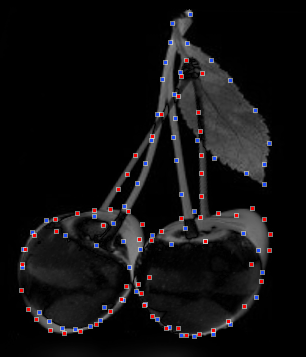
\includegraphics[width=6cm,keepaspectratio=true]{./cherries-match.png}
\caption{Dopasowanie \texttt{cherries} do \texttt{cherries6}}
\end{figure}


\begin{figure}\centering
\subfloat[Jabłko]{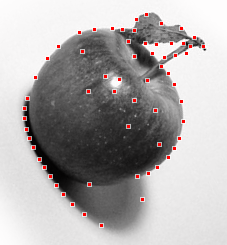
\includegraphics[width=5cm,keepaspectratio=true]{./apple-mod-pois.png}}
\subfloat[Wisienki]{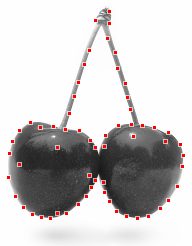
\includegraphics[width=5cm,keepaspectratio=true]{./cherries-pois.png}}
\subfloat[Trójliterówka]{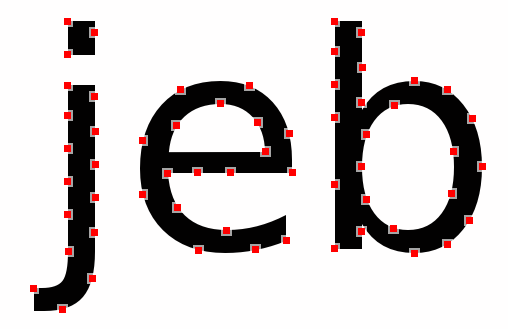
\includegraphics[width=5cm,keepaspectratio=true]{./jeb-pois.png}}
\caption{Wybrane obrazy testowe}
\end{figure}

\end{document}
